\chapter{Konvenční prostředky a polygonizace}
\label{chap:konvencni prostredky a polygonizace}
	Existuje celá řada konvenčních nástrojů, kterými lze řešit polygonizaci. Oblast GIS je známá značným množstvím kvalitních nástrojů s otevřeným zdrojovým kódem. Můžeme tak nalédnout do implementace jednotlivých softwarových řešení. Výhodou je i velká komunita, která vždy ochotně poradí. Mimo jiné jsou zde i komerční zástupci, kteří nám možnost nahlédnout do zdrojového kódu zpravidla nenabídnou. Zato by nám měli poskytovat uživatelskou podporu, za kterou zákazník samozřejmě platí koupí softwaru.
	
	Mohlo by se zdát že nástrojů existuje celá řada, tak proč vytvářet nástroj nový? Jedná se zde především o spolehlivost a jednoduchost. Jak u komerčních, tak u open source nástrojů je s nadsázkou téměř tradicí, že po přechodu na vyšší verzi nějaké komponenty přestanou fungovat a končí na neočekávaných chybách. Výjimkou nejsou ani nástroje pro polygonizaci.
	
	Zmíníme zde tedy nejvýznamější zástupce z oblasti GIS a ukážeme, které nástroje z těchto softwarů lze pro polygonizaci využít.
	
\section{ArcGIS Desktop}
	ArcGIS je vyvíjený společností Esri, v současné době se jedná o jeden z nejvyužívanějších nástrojů v oblasti GIS. Jedná se o placený software za který nekomerční uživatel v současné chvíly zaplatí 100 dolarů ročně. Používat tento nástroj tedy pouze pro polygonizaci by bylo nesmyslné, ovšem pokud uživatel již tímto softwarem disponuje je toto jedna z možností.
	
\subsubsection{Feature to Polygon}
	\textit{Feature to Polygon} je nástroj sloužící pro tvorbu polygonů. Jako vstupní data mohou být použity linie i polygony. Výstupní polygony z tohoto nástroje na testovacích datech byli korektní, ovšem při větším množství vstupních linií testovaný nástroj končil chybou. Nutno podotknout že u různých verzí softwaru se může nástroj chovat jinak.

\begin{figure}[h]
  \centering
  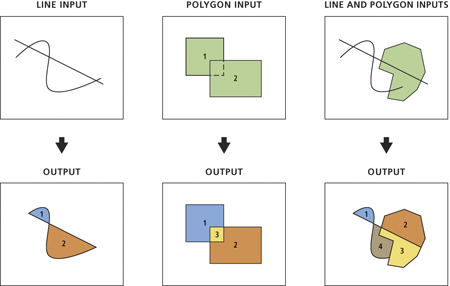
\includegraphics[width=10cm]{./pictures/5.1/feature_to_polygon.png}
  \caption{Ilustrace vstupu a výstupu nástroje Feature to Polygon. Převzato z~\cite{arcgis}.}
  \label{fig:feature_to_polygon}
\end{figure}

\begin{figure}[h]
  \centering
  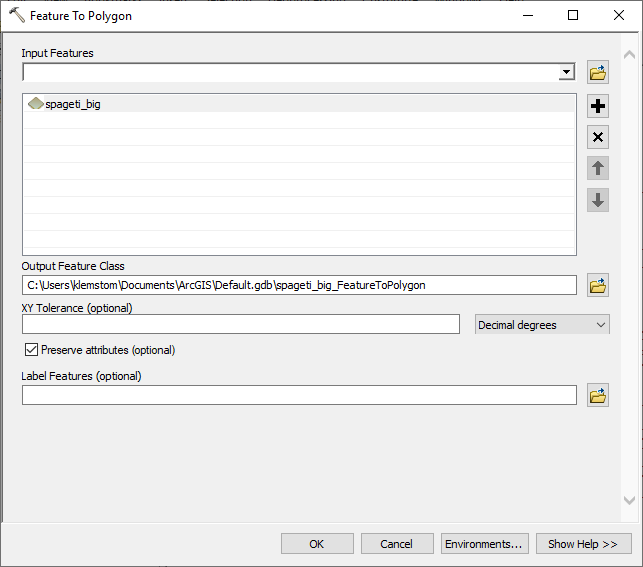
\includegraphics[width=10cm]{./pictures/5.1/feature_to_polygon-1.png}
  \caption{Rozhraní nástroje Feature to Polygon v softwaru ArcGIS Desktop.}
  \label{fig:feature_to_polygon-1}
\end{figure}


\subsubsection{QGIS Desktop}
	Přímím konkurentem softwaru ArcGIS Desktop je bezpochyby vydařený QGIS Desktop. Jedná se o nástroj vyvýjený komunitou pod záštitou OSGeo. Je šířen pod copyleftovou  licencí \textit{GNU General Public License}, tudíž máme volný přístup ke zdrojovému kódu aplikace dostupných v online repozitářích. To nám umožňuje nahlížet do výpočetních algoritmů, které jsou v případě QGis psány v programovacím jazyce \textit{C++} a \textit{Python}, narozdíl od komerčních nástrojů, které si implementaci často chrání. Výstup z nástroje byl opět validní. Narozdíl od nástroje z ArcGIS Desktop se ovšem podařilo zpracovat i větší množství dat.

\begin{figure}[h]
  \centering
  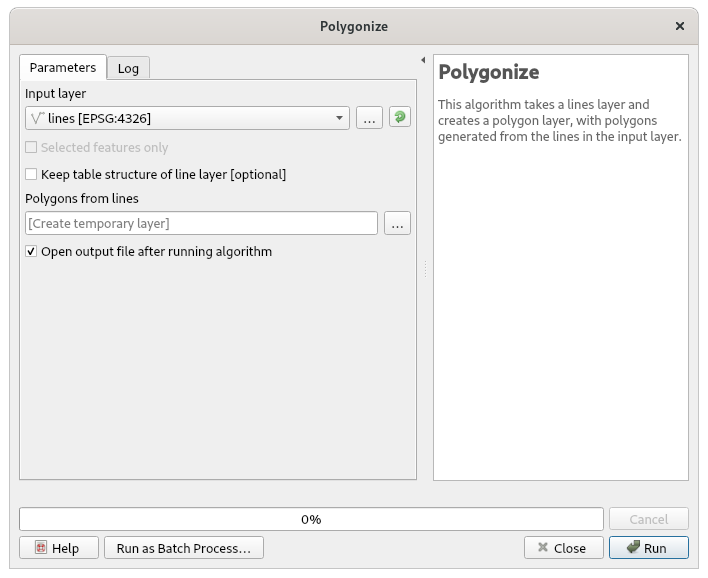
\includegraphics[width=10cm]{./pictures/5.1/polygonize.png}
  \caption{Rozhraní nástroje Polygonize v softwaru QGIS Desktop.}
  \label{fig:polygonize}
\end{figure}

\subsection{PostGIS}
	Obdobně byl testován i nástroj PostGIS. Zde už se nejedná o desktopovou aplikaci jako tomu bylo u výše testovaných softwarů. PostGIS je nadstavba pro objektově-relační databázi PostgreSQL. Jedná se tedy o rozšíření databáze o podporu geografických objektů a funkcí. Je často využíván k uchování geografických dat a analýz nad nimi, jelikož přebírá veškerou funkcionalitu databázových serverů. Nutno podotknout že PostGIS využívá pro většinu svých operací knihovnu \textit{GEOS} psanou v programovacím jazyce \textit{C++}, kterou následně poskytuje uživateli přes standardní dotazovací jazyk SQL.
